%\linenumbers*
\chapter{THE PROBLEM IN CONTEXT}
\label{sec:PROBLEMINTHECONTEXT}

\section{Introduction}
\label{sec:Rationale}
Soil is an important resource for the survival of the human race and is a
central component of environmental systems, together with water, air and
radiation from the sun. Undoubtedly, soil is one of the essentials for life on
Earth. Scientists have investigated various soil properties to ensure good
yields of crops, fibre and fuel \citep{cresser1993-192}. However, soils do not
necessarily always provide ideal conditions for plant growth. Many soil
processes can constrain plant growth: soil hydrology is fundamental for most of
these \citep{hudson1971-320, evans1980-mechanics, kirkby1980-1,
morgan1995-soil}. Among the most serious is soil erosion by water.

Globally, soil erosion by water is a serious present-day environmental problem
and its consequence is subject to extensive investigations
\citep{kirkby1980-1,morgan1995-soil}. Previously published simulation studies of
the effects of future climate change upon erosion indicate that, under land
usages that leave the soil unprotected, even minor increases in rainfall amounts
are likely to result in disproportionately large increases in erosion
\citep{kirkby1980-1, favis-mortlock1995-365}.

Soil erosion rates may be expected to change in response to changes in climate
for a variety of reasons \citep{pruski2002-climate}, the most direct of which is
the change in the erosive power of rainfall
\citep{favis-mortlock1996-529,williams1996-381,favis-mortlock1999-329,
nearing2001-229,pruski2002-climate}.
%Soil erosion responds both to the total amount of rainfall and to
%differences in rainfall intensity, however in some situations (e.g. when
%soil is already saturated) the dominant factor appears to be rainfall
%intensity and energy rather than rainfall amount alone.
Existing studies however almost invariably make the simplifying assumption that
distributions of future rainfall intensities remain unchanged from the present
\citep{favis-mortlock1995-265,favis-mortlock1995-365,favis-mortlock1999-329,
pruski2002-climate,pruski2002-7,o'neal2005-165}. This is unlikely to be the
case. Intensities may change and/or the frequency of occurrence of
high-intensity events may change \citep{karl1995-217,houghton1996-climate,
watson1998-517,karl1998-231,osborn1998-505,osborn2002-1313}. Any
increases in the occurrence of high-intensity rainfall---even without any
associated increases in rainfall amounts---may well increase runoff, and hence
erosion rates \citep{kirkby1980-1, morgan1995-soil, parsons2000-723}. Future
climate change will certainly affect rainfall intensities but our ability to
forecast future intensities is limited by the shortcomings of General
Circulation Models (GCMs) \citep{favis-mortlock1995-365}.

Few studies have attempted to quantify changes in future rainfall intensity
\citep{karl1995-217,houghton1996-climate,watson1998-517,karl1998-231,
osborn1998-505,osborn2002-1313}. Results from these studies suggest that more
(or similar) rainfall than at present will occur on fewer raindays---implying an
increase in the frequency of heavy rainfall. If these predictions are correct,
the implication for future erosion rates are clear. For these reasons, there is
a urgent need for greater understanding of future rainfall intensity changes in
order to improve the ability of soil erosion prediction.

This thesis, therefore, aims to address some of the issues involved in
predicting future soil erosion as a response to future changes of rainfall
intensity. More detailed aims and issues associated with achieving those aims
are presented at the end of Chapter 2. Prior to Chapter 2, topics that are
related to soil erosion processes, rainfall intensity, climate changes and
erosion prediction models are discussed in the following sections.

\section{Soil Erosion Processes}
\label{sec:SoilErosionProcesses}

\subsection{Introduction}
\label{sec:ErosionProcessesIntroduction}

\begin{quote}
  \begin{quote}
    ``Erosion by water is the redistribution and removal of the
upper layers of the soil, both by the action of falling rain, and by water
flowing over the soil during and after rain or following snowmelt.''
\citep{favis-mortlock2002-452}
  \end{quote}
\end{quote}

The erosion of soil by water and wind is a naturally occurring process, which is
commonly accelerated by human activity. However, when soil erosion occurs at a
greater rate than the rate of soil formation, soil erosion is considered as an
environmental problem. Soil erosion is a ubiquitous problem that threatens an
important and non-renewable resource such as the agricultural land that is
suitable for cultivation (on-site impact) \citep{boardman2003-176}. In addition
to removing a valuable resource, soil erosion leads to increased sediment input
to nearby watercourses, resulting in, for example, the silting-up of dams and
contamination of drinking water (off-site impact)
\citep{mejia1994-331,kitchen1998-179}.

Soil erosion problems can be viewed in three different ways
\citep{kirkby1980-312}. Firstly, in the broadest view, soil erosion can be
compared with other processes of landscape denudation. When and where it is the
most rapid process, soil erosion should be recognised as the dominant problem.
This view leads to the question of what erosion rates can be tolerated in the
long-term. Secondly, a narrower overview examines soil erosion with its
immediate climatic and vegetational controls. This then leads to the question as
to how well the processes involved in raindrop impact, flow generation, and
sediment resistance are understood. Thirdly, soil erosion can be considered in
relation to its broad patterns in time and space. However, the reasons for the
temporal and spatial distributions of soil erosion are only partially understood
\citep{quine2002-55,gomez2005-143,wakiyama2010-993}.

Soil erosion by water is most active where rainfall cannot infiltrate the soil,
but flows over the surface. As the flow travels down a hillslope, it is able to
carry soil materials away mainly by shear stress although other sub-processes
also contribute \citep[see also Figure
\ref{fig:kinnell}]{kinnell2000-discourse,kinnell2005-2815}. In some
cases, only an hour or two of contact time with the surface soil is needed to
carry away an appreciable amount of material. Thus, where overland flow is
dominant, soil erosion by water is likely to be the main process of landscape
denudation. When a large depth of water flows rapidly over the surface with
correspondingly large hydraulic forces, soil erosion acts catastrophically.
These conditions are most commonly found in semi-arid areas, but fields cleared
for agricultural purposes are also subjected to erosion in almost any climate,
which can on occasion be severe \citep{boardman2001-346,boardman2003-176}.

Semi-arid areas are very sensitive to small natural changes in climate and in
such areas it is difficult to separate natural from man-induced changes in
erosion rates. However, even in temperate-humid areas increased erosion
resulting from farming can be sensitively dependent on the extent of the change
in vegetation cover, the total rainfall at periods of low cover, and the
intensity of the rains.

Therefore, two distinct types of area appear to be at great risk of soil
erosion. The first are semi-arid areas, and the second are locations in
temperate areas that have been stripped of vegetation for crop cultivation. A
soil erosion rate can reach at its maximum where intense rainfall occurs during
the period of lowest vegetation cover. This is normally the case in semi-arid
climates or in temperate areas which have been left bare at the time of the
heaviest annual rainfall. In such cases, when the rainfall increases, soil loss
increases, so that the erosional peak tends to be synchronised with the rainfall
peak and this relationship becomes more distinctive when the soil becomes more
unprotected.

When soil erosion problem is to considered, it also is worthwhile to take
long-term effects of soil erosion into consideration. For example, when soil
erosion occurs at a rate of one millimetre per year, it might not have apparent
effect in a human lifetime. However, over a longer-term, the effect can be
considerable. To put this into perspective, topsoil of 15 cm thickness in
general would be completely removed after 150 years if erosion rates stay as
high as 1 mm/year in average with no additional soil formation in the area.
Topsoil contains a high proportion of soil organic matter and the finer mineral
fractions, which provide water and nutrient supplies for plant growth. This may
look as an oversimplification of the erosion process and soil formation, but it
gives us an idea of the long-term effect of soil erosion.

%When soil erosion occurs at a rate of, for example, one millimetre per year, it
%might have little apparent effect in a human lifetime. However, over a
%longer-term, effects can be considerable. This is because erosion continually
%removes the topsoil (e.g., topsoil of 15 cm thickness would be completely
%removed after 150 years if erosion rates are higher as 1 mm/year without
%renewal) which contains a high proportion of soil organic matter and the finer
%mineral fractions, which provide water and nutrient supplies for plant growth.

\subsection{Rainfall}
\label{sec:RainfallCharacteristics}

\subsubsection{Raindrop Splash}
% Raindrop Impact Induced Erosion (need to put more appropriate title)
\label{sec:RaindropSplash}

The process of erosion by water is a two-phase process: detachment and transport
\citep{morgan1995-soil}. Individual soil particles are detached from the soil
mass by the impact of raindrops. The erosive power of raindrops weakens and
loosens the soil surface, and flowing water transports the soil particles
\citep{kinnell2000-discourse}. When sufficient transporting energy is no longer
available, a third phase, deposition, can occur.

\begin{figure}[htbp]
  \centering
  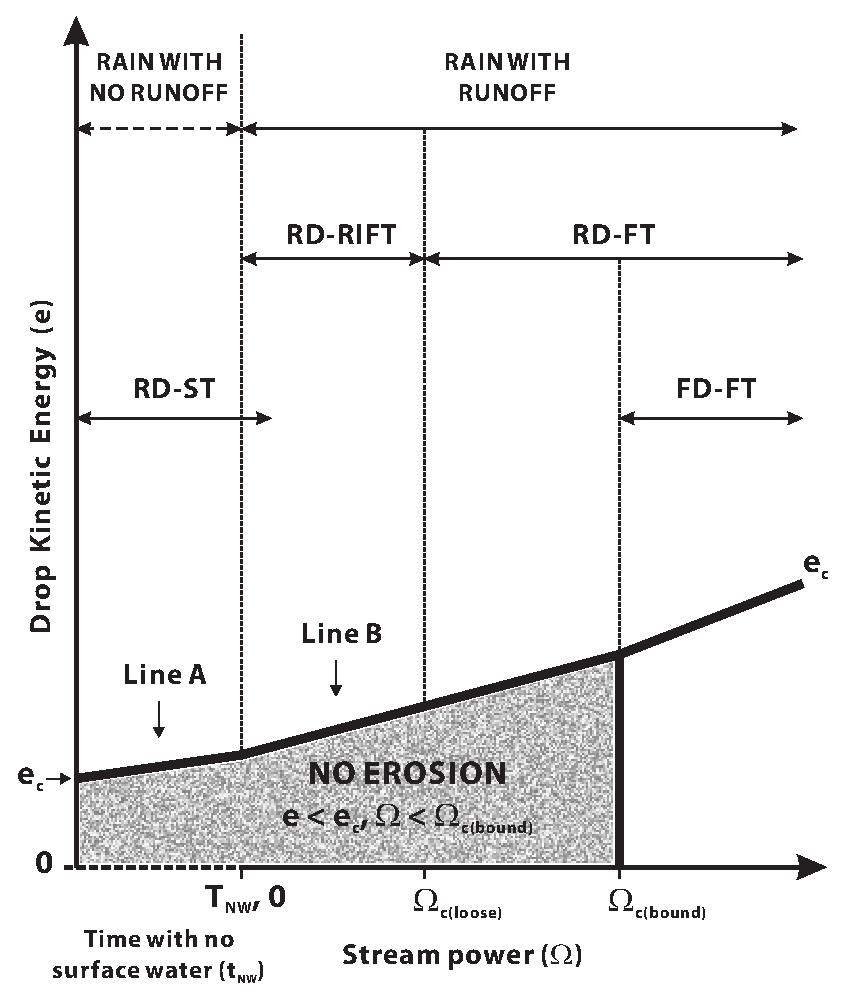
\includegraphics[width=0.70\textwidth]{./img/kinnell}
  \caption[Detachment and transport processes]{Detachment and transport
processes associated with variations in raindrop and flow energies. $T_{NW}$:\
total time when rain falls and there is no surface water. $e_c$:\ critical
raindrop energy to cause detachment; raindrop-induced erosion occurs when drop
energy is equal or greater than $e_c$. Line A:\ $e_c$ when raindrops are
detaching soil particles from the soil surface prior to flow developing. The
slope on this line is used to indicate increasing resistance to detachment
caused by, for example, crust development. Line B:\ $e_c$ when raindrops are
detaching soil particles from the soil surface when flow has developed. The
slope on this line is used to indicate increasing utilization of raindrop energy
in penetrating the flow when flow depth increases as flow power increases.
$\Omega_{c\textrm{(loose)}}$:\ critical stream power required to transport loose
(pre-detached) soil particles. $\Omega_{c\textrm{(bound)}}$:\ critical stream
power required to detach particles bound within the soil surface (held by
cohesion and interparticle friction). RD-ST:\ raindrop detachment and splash
transport. RD-RIFT:\ raindrop detachment and raindrop-induced flow transport.
RD-FT:\ raindrop detachment and flow transport. FD-FT:\ flow detachment and flow
transport\citep[From][]{kinnell2005-2815}.}
  \label{fig:kinnell}
\end{figure}

Raindrop splash distributes soil particles radially away from the site of
detachment. The raindrop detachment-splash transport (RD-ST in Figure
\ref{fig:kinnell}) process is effective where rainfall intensities are high, for
example, as a result of convective rainstorms. However, splash transport (ST) is
a generally inefficient transport mechanism. If the soil has virtually no slope,
soil particles splashed away from the point of impact are replaced by soil
particles detached by other raindrops in the surrounding area
\citep{kinnell2000-discourse,zartl2001-25}. Even if the soil surface has a
slope, net downslope transport by raindrop splash alone is generally small
\citep{kinnell2001-749}.

When water flows start to build up, the soil surface becomes protected from
direct raindrop impact, and another transport mechanism begins to dominate.
Raindrops with sufficient kinetic energy to penetrate through the flow may
detach and lift soil particles into the flow, which then carries them downstream
until it loses sufficient transporting energy to carry the particles. Soil
particles transported by the flow then fall back to the soil surface of lower
grounds. This transport process is termed Raindrop-Induced Flow Transport (RIFT
in Figure \ref{fig:kinnell}) \citep{kinnell1990-497}. While RIFT is more
efficient than ST, it still requires numerous raindrop impacts to move soil
particles downstream.

As rain continues, thin surface water flows become capable of moving loose soil
material on the top of the surface, but might not be capable of detaching soil
material from the soil mass. In many cases, soil particles are detached by the
help of raindrop impacts, and carried away downstream without the need for
raindrops to be involved in the transport process. This raindrop detachment-flow
transport (RD-FT) process is more efficient than RD-RIFT. In a typical field,
both RD-RIFT and RD-FT occur simultaneously in the same flows.

When the critical stream power ($\Omega_{c\textrm{(bound)}}$) for flow to detach
soil particles from soil mass exceeds stream power ($\Omega$), flow detachment
(FD) occurs \citep{kinnell2000-discourse}. Once soil materials are detached and
transported by flow (FD-FT), erosional channels are generated (Figure
\ref{fig:kinnell}). As these channels develop and increase in size to become
large rills and possibly even gullies, processes such as gravitational collapse
of channel walls and heads become important \citep{boardman2003-165}.

\subsubsection{Rainfall Intensity} % Rainfall Intensity Patterns?
\label{sec:RainfallIntensity}

The erosive power of rainfall has long been appreciated by studies on soil
erosion \citep{musgrave1947-133,wischmeier1958-rainfall}. Nevertheless,
obtaining information on rainfall intensity for soil erosion is very much
problematic. One way of measuring rainfall intensity would be measuring size,
distribution and velocity of raindrops, so that the kinetic energy of the
rainfall can be calculated \citep{cerda1997-169,lascelles2000-709}. This can be
seen as a `bottom-up' approach. Another method would be simply to measure
rainfall amount and duration, so that intensity can be obtained by dividing
rainfall amount by duration (i.e. rainfall amount per unit time)
\citep{osborn1998-505}. This is a `top-down' approach. However, both approaches
have their own shortcomings
\citep{parsons2000-723,schuur2001-1019,garcia2001-675}.

Although rainfall intensity plays a very important role for soil erosion, it is
important to recognise that the vital variable for soil erosion by splash is not
rainfall intensity itself, but rainfall energy. This rainfall energy varies in
association with rainfall intensity. As raindrops increase in size, their
terminal velocity increases. This increases the kinetic energy of raindrops. The
total kinetic energy of rainfall also increases with increasing number of
raindrops during a given time. The total kinetic energy of rainfall may be
estimated from the distribution of raindrop size and number of raindrops during
a storm. The accuracy of this estimation is, however, limited by natural
variations in rainfall characteristics \citep{vandijk2002-1}. Yet, in natural
rainfall events, the relationship between rainfall intensity and energy is
neither so clear, nor simple. Despite this, simple assumptions about the
rainfall intensity-energy relationship are often made in studies on soil
erosion, in particular, modelling studies, as rainfall intensity is the
only easily modifiable control on rainfall energy in such studies
\citep{laflen1997-96,morgan1998-389}.

\citet{parsons2006-68} ran a laboratory-based rainfall simulation
experiment to determine the implications of temporal variation of rainfall
intensity for rates of soil loss. He found that erosion is least for the
constant-intensity storms. This is highly significant because soil-erosion
models are typically calibrated using data obtained from constant-intensity
experiments. Moreover, storm pattern does not appear to affect the volume of
runoff, but it does affect the quantity of eroded sediment. In particular, the
constant-intensity storm patterns are associated with low erosion rates. Storm
pattern also affects the size-distribution of the eroded sediment.
\citet{parsons2006-68} therefore concludes that the relationship between
rainfall energy and interrill erosion is more complex than is currently assumed
in process-based models of soil erosion.

Other studies also note that there are complex interactions between raindrop
size, velocity and the duration of rain, which control the erosive power of
rainfall \citep{kinnell1981-153,brandt1990-687,salles1999-545,vandijk2002-1}.

\subsection{Soil Type}
\label{sec:SoilType}

Soil erodibility is an estimate of the resistance of the soil to erosion, based
on the physical characteristics of each soil \citep{morgan1995-soil}. Although
erodibility varies with soil texture, aggregate stability, shear strength,
infiltration capacity and organic and chemical contents, soils with high
infiltration rates, higher levels of organic matter and improved soil structure
have a greater resistance to erosion, in general \citep{morgan1995-soil}.

Erodible soils have restricted clay content \citep{bryan2000-385}. Soils with
more than 30--35\% clay are generally coherent and form stable soil aggregates,
which are resistant to raindrop impact and splash erosion
\citep{evans1980-mechanics}. Clays often have rough surfaces to store much
water, and are resistant to sheet and rill erosion. Sands and coarse loamy
sands, on the other hand, have high infiltration rates and resistant to erosion,
and even if this is exceeded, sands (more than 0.3 mm diameter) are not easily
eroded by flowing water or by raindrop impact
\citep{evans1980-mechanics,marshall1996-soil}.

Sandy soils are however more erodible than clayey soils because the aggregates
of these sandy soils slake more readily and seal the soil surface
\citep{lebissonnais1996-425}. Loamy soils are also particularly at risk of
sealing \citep{ramos2000-398}.

After cultivation, the soil surface becomes rough. The amount of water, which
can be stored on the surface before runoff takes place, is thus large at this
time. Surface roughness is least after drilling and rolling of the seedbed, and
differences between soil types are smallest \citep{robinson1992-151}. For
similar soil types, the timing of cultivation can affect the storage volume, for
example, a clay surface prepared in winter can have more than twice as much
storage volume as a surface prepared in spring \citep{evans1980-mechanics}.

Moreover, stony soils are generally less vulnerable to erosion as the surface
stones not only protect the soil, but also increase infiltration by providing
larger pores between stones
\citep{agassi1991-565,poesen1994-1,defigueiredo1998-81}. However, when rock
fragments are well-embedded in a surface seal, a positive relation for runoff
and sediment yield is found \citep{poesen1992-451}. A negative relation occurs
either where rock fragments are partly embedded in a top layer with structural
porosity or where the rock fragments rest on the surface of a soil having either
textural or structural pore spaces \citep{poesen1992-451}.

\subsection{Topography}
\label{sec:Topography}

There are two aspects of topography that affect erosion: slope angle and length.
Normally, erosion would be expected to increase as the slope steepness increases
\citep{liu1994-1835}. Soil erosion by water also increases as the slope length
increases because of increases in velocity and volume of runoff
\citep{liu2000-1759}. Water depth increases with downslope distance so that
interrill soil erosion is affected by slope length \citep{gilley1985-154}.
Water depth then affects soil detachment and overland flow sediment transport
capacity \citep{gilley1985-147}. Slope angle is also closely related to the
effectiveness of splash erosion \citep{kinnell2000-discourse,vandijk2003-153}.

The location of downslope is an important factor that determines the
development of rills on a hillslope. However, there is another factor that is
closely related to the dynamics of initiation and growth of rills. The
minute variations of soil surface topography, also known as microtopography, can
play an important roll on this ``rill competition''.

Microtopography is not temporally static because erosional processes will
continuously modify the surface of soil during a rainfall event. As a
result, runoff during the latter part of the event will flow over a soil
surface that has been modified and different from the surface earlier in the
rainfall. Thus, erosive modification of microtopography constitutes a feedback
loop which might be expected to operate in a positive sense. The most
`successful' rills (i.e. those conveying the most runoff) will modify the local
microtopography to the greatest extent, and so will most effectively increase
their chances of capturing and conveying subsequent runoff.

\citet{favis-mortlock2000-2173} previously recognised the importance of
microtopography
in the initiation and the development of rills, and developed a erosion model,
RillGrow, using a self-organising dynamic systems approach. More about RillGrow
is included in Section \ref{sec:ModelDescriptionRillGrow}.
%******you need to mention also something about microtopograghy, at the mm to cm
%scale, about how this is important in (among other things) determining the
%location of preferential flow paths and so of rills.

\subsection{Land Use}
\label{sec:LandUse}

Soil erosion potential is highest where the soil has no or very little
vegetative cover. Vegetation cover protects the soil from direct raindrop impact
and splash, and tends to slow down surface runoff. On a field with complete
vegetation cover, runoff and erosion are comparatively small, often less than
5\% of runoff and 1\% of erosion from bare soil, respectively
\citep{braskerud2001-1447,rey2003-549}. One reason is because the infiltration
rates of the vegetated field are relatively higher than those on bare soils as
the field often has a better soil structure and more stable aggregates
\citep{robinson2001-1}. When runoff does take place, the leaves and roots of
plants inhibit the flow by reducing the velocity of the flow
\citep{braskerud2001-1447,rey2003-549}. On soils with less than 70\% vegetation
cover, runoff and erosion increase rapidly when rainfall occurs
\citep{favis-mortlock1996-529}. Under less than 20--30\% vegetation cover,
runoff and erosion are related to the amount of bare ground, increasing as the
proportion of bare ground increases \citep{favis-mortlock1996-529}.

The effectiveness of any crop management system against soil erosion by water
also depends on how much protection is available at various periods during the
year, relative to the rainfall amount that falls during these periods. In this
respect, crops which cover for a major portion of the year (e.g., alfalfa or
winter cover crops) can reduce erosion much more than can crops (e.g., row crops
) which leave the soil bare for a longer period of time and particularly during
periods of intense rainfall \citep{zhang1995-1069,zhang1995-1079}.

%\subsection{Rill and Interrill Erosion}
%\label{sec:RillAndInterrillErosion}
%
%Rills are initiated at a critical distance downslope where overland flow
%becomes channelled.
%
%Interrill erosion is due to detachment and transport by raindrop impact and
%overland flow. Interrill erosion has been shown to be approximately
%proportional to the square of the rainfall intensity \citep{watson1986-97}.
%In addition to rainfall intensity, interrill erosion is related to slope
%\citep{watson1986-97}.

\section{Soil Erosion and Rainfall Intensity}
\label{sec:RainfallIntensityAndSoilErosion}

This section provides examples of some notable erosion events which are
documented in selected publications.



\paragraph{South Downs, East Sussex, UK, October 1987
\citep{boardman1988-333}}
\label{sec:SouthDownsOctober1987}

Heavy rainfall on 7 October 1987 and subsequent storms resulted in soil losses
over 50 m$^3$/ha\ on several fields and over 200 m$^3$/ha\ on one field in the
eastern South Downs \citep{boardman1988-333}. Monthly rainfall totals at
Southover, Lewes, were 54.3 mm for September and 270.9 mm for October 1987.
Rainfall recorded at Southover, Lewes, on 7 October 1987 was 50.2 mm with a
maximum short period intensity of 6.7 mm/h\ for 5.5 hours including 40 mm/h\ for
15 minutes.

Substantial rills or gullies were formed by the rainfall event on 7 October
1987. As a result of this, following rainfalls as low as 7 mm caused runoff and
erosion \citep{boardman1988-333}.
Although there are no event-by-event records available for soil losses, it is
evident that the rainfall on 7 October 1987 played an important role, by
contributing to rill or gully generation, on  soil erosion in the area. However,
the main factors responsible for the severe erosion were land use and farming
practices.

%%%%%
\paragraph{Vicrello, Tuscany, Italy, May 1994 \citep{torri1999-131}}
\label{sec:VicrelloVolterraTuscany}

A rainfall depth of 77.8 mm fell on a field plot with a bare soil in Vicrello,
Tuscany, Italy \citep{torri1999-131}. The storm lasted for over 28 hours and
caused a soil loss of 126.2 t/ha. Maximum intensity averaged over 10 minute was
120 mm/h.

\paragraph{Hadspen, Somerset, UK, May 1998 \citep{clark2000-17}}
\label{sec:HadspenSomersetUK}
Total rainfall amount of 47.6 mm fell in Hadspen, Somerset, UK on 13 May 1998
\citep{clark2000-17}. Most rain fell between 2115 GMT to 2130 GMT reaching
rainfall intensity of $>$100 mm/h. In Nettlecombe Hill and Higher Hadspen,
ploughed fields on slopes with 2--11\textdegree\ eroded 1.412
tonnes/m$^3$ and 1.312 tonnes/m$^3$ as dry bulk density, respectively.
Because of the difficulties involved in measuring soil loss amount directly,
\citet{clark2000-17} took survey to estimate the volume of soil that was cleared
from the site and dumped into a nearby field. Then, samples from soil was taken
and the dry bulk density was determined. Total soil loss from two area was 60.6
tonnes and 11.5 tonnes respectively.

\paragraph{Ashow, Warwickshire, UK, August 1999 \citep{harrison1999-143}}
\label{sec:AshowWarwickshireUK}
On 20 August 1996 in Ashow, Warwickshire, the storm commenced at 1930 BST.
Rainfall intensity was low until 2030 BST when 24.5 mm of rain fell in 30 min
and a total of 33.5 mm fell before midnight.

One of two fields in the catchment was planted with oilseed rape eight days
before the storm. The field was ploughed and power-harrowed, and then seed
drilled with a low ground pressure buggy. It was subsequently rolled by a
tractor with low ground pressure tyres. The other field was harvested of wheat
and barley, and then rough ploughed, the soil clods being broken up using
rotating discs.

Extensive erosion of top soil occurred, followed by the development of gullies
and rills by overland flow during the storm. Approximately 790 tonnes of
sediment was eroded from the two fields excluding the sediment that reached
nearby river (River Avon, UK). Average sediment yields was 49.7 t/ha which is
equivalent to the average ground lowering of 3.8 mm from the site.

\paragraph{Northern Ethiopia Highlands, 1998-2000 \citep{nyssen2005-172}}
\label{sec:NorthernEthiopiaHighlands}

Rainfall intensity in Northern Ethiopia Highlands was monitored using a tipping
bucket rain gauge during 1998-2000 \citep{nyssen2005-172}. Overall rain
intensity in the area is low. 88\% of total rain volume falls with an intensity
$<$30 mm/h. Most storms have a low intensity with a brief high intensity part.
This high intensity can be observed at the beginning, in the middle or at the
end of the storm.

Although area-averaged intensity was low in this area, it was found that maximum
rain intensity at individual locations exceeded by far the threshold values for
excessive rain (see Table 5, \citealp{nyssen2005-172}). Rainfall intensities
beyond these thresholds were known to cause $>$50\% of total soil losses
\citep{krauer1988-rainfallerosivityand}. Large rain erosivity in the area is due
to larger median volume drop diameters ($D_{50}$) than those reported for other
regions of the world, rather than due to high intensity.

Despite the low rainfall intensity, presumably large proportions of soil may
have been lost from the area. The article only implies the erosion event. Also,
no actual soil loss amount was presented.

%%%%%
\paragraph{South Downs, East Sussex, UK, October 2000
\citep{boardman2001-346}}
\label{sec:SouthDownsOctober2000}

Exceptional rainfall in October and November 2000, especially a 24-hour fall of
about 100 mm, led to extensive erosion and property damage
\citep{boardman2001-346}. The rainfall was typical of frontal, low-intensity
events that usually occur in British winters but it lasted for a longer period
than usual period. In a 24-hour period prior to 09:00 on 12 October (i.e.\ 11
October rainday), a total rainfall of 89.9 mm was recorded
\citep{boardman2001-346}.
In a 10-hour period of continuous rainfall (23:00--09:00) 63.8 mm fell with a
maximum intensity of 11.4 mm/h\ and a maximum short-period intensity of 3.6
mm/min\ (i.e.\ 216 mm/hr) \citep{boardman2001-346}.

Rainfall of 100 mm in 24 hours has a return period of well over 100 years and a
intensity of 11 mm/h is to be expected every year \citep{boardman2001-346}. This
means that the rainfall on 11 October 2000 has a rainfall intensity that is
commonly observed in the area, but the total amount and duration are very
unlikely in the area. It is noted that high intensity rainfall within prolonged
low intensity rainfall at the time of year when the agricultural land is most
vulnerable may result in extensive erosion events.

On one field from the studied site, a gully up to 1.5 m deep, 0.5 m wide and
more than 200 m long was cut by runoff on 11 October 2000. Because no erosion
measurement was taken during the rainfall event, total erosion amount is
unknown for the specific event on 11 October 2000 but severe erosion and muddy
flood occurred on the day. 

\paragraph{Synthesis}
The events presented above are few examples of rainfall events that were
followed by soil erosion events. Although they are subjectively selected, this
is not an either comprehensive or limited list.

These cases give an idea of the diversity of soil erosion responses
to different (i.e.\ high or low) rainfall intensities. Severe soil erosion
events do not necessarily always occur with rainfall events with high rainfall
intensity. Rainfall events with low intensity can also produce soil erosion.
This is because sometimes (and quite often) other erosion-affecting factors such
as the timing of a rainfall event may play more important roles than rainfall
intensity. Thus, it would be difficult to compare these events presented in this
section directly in order to identify the effect of rainfall intensity.

Also, these case studies presented here show that studies of rainfall events
that were followed by sever erosion events do not always have measurements for
the erosion. This is an importance issue. The difficulties that arise from
monitoring and modelling soil erosion often start from finding ``right''
observational data. This would be the first obstacle that one may have to face
when doing simulation studies on soil erosion.


\section{Rainfall Intensity and Climate Change}
\label{sec:RainfallIntensityAndClimateChange}

Many studies using GCMs predict an increase in global average precipitation in
response to global warming induced by greenhouse gases
\citep{houghton1996-climate,jones2001-1337,ipcc2001-881,ipcc2001-1032,
ipcc2007-impact,ipcc2007-physical}. This increase in global average
precipitation has been based on the assumption that an increasing global-mean
temperature will intensify the hydrological cycle
\citep{nearing2005-131}. The IPCC reported that there has been a very
likely increase in precipitation during the 20th century in the mid-to-high
latitudes of the Northern Hemisphere \citep{ipcc2001-881,ipcc2007-physical}.
Climate models are also predicting a continued increase in intense precipitation
events during the 21st century \citep{ipcc2001-1032,ipcc2007-impact}.

In addition, there has been a number of investigations using observed data
that provided some evidences for a significant increase in extreme precipitation
\citep{karl1995-217,karl1998-231,osborn2000-347,osborn2002-1313}.
\citet{karl1995-217} and \citet{karl1998-231} observed increases in extreme
precipitation (greater than 50 mm per day) in the United States using historical
data over the period 1910--1996. \citet{osborn2000-347} and
\citet{osborn2002-1313} also observed an increasing trend in intense daily
precipitation over the period 1961--2000 in the United Kingdom. They found that,
on average, precipitations were becoming more intense in winter and less intense
in summer.

The findings by \citet{osborn2000-347} and \citet{osborn2002-1313} are generally
consistent with the results from the GCM simulations
\citep{jones1997-265,jones2001-1337}. However,
\citet{ipcc2001-1032,ipcc2001-881} indicated that potential changes in intense
rainfall frequency are difficult to infer from global climate models, largely
because of coarse spatial resolution. The ability of GCM integrations and
operational analyses to simulate realistic precipitation patterns, spatially and
seasonally, is also generally not as good as the ability to predict temperature
\citep{mcguffie1999-1}. The likelihood of finding real trends in the frequency
of extreme events becomes lower the more extreme the event
\citep{frei2001-1568}. The same authors demonstrate this by applying known
trends in the scale parameter to synthetic data series, and then attempt to
identify statistically significant trends in the frequency of various extreme
events.

%******$Summarise what are those physical reasons in \citealp{trenberth2000-12}.

There are various physical reasons (see \citealp{trenberth2000-12}) why a large
increase in the magnitude of heavy precipitation may occur with only a
correspondingly small increase in mean precipitation. It is even possible that
heavy precipitation occurrence could increase when mean precipitation decreases,
if there is a more radical change in the precipitation distribution
\citep{osborn2002-1313}.

A study by \citet{nearing2001-229} estimated potential changes in rainfall
erosivity in the United States during the 21st century under climate change
scenarios. He concluded that, across the United States over an 80 year
period, the magnitude of average changes in rainfall erosivity was 16--58\%.
This variability in the magnitude was due to the method (two GCM models and
two scenarios) that he used to predict the changes in rainfall erosivity.
Regardless of which method was used, he suggested that changes in erosivity will
be critical at certain locations.

In order to run a soil erosion model such as WEPP (Water Erosion Prediction
Project, See Section \ref{sec:WaterErosionPredictionProjectWEPP} for more
details), for example, various weather parameters for each day of the
simulation period are required \citep{flanagan1995-usda}. These weather
variables (e.g. rainfall depth and duration, peak storm intensity and time to
peak, minimum and maximum temperatures, dew point temperature, solar radiation,
wind speed and direction) can either be generated by CLIGEN (CLImate GENerator,
See Section \ref{sec:ClimateGeneratorCLIGEN} for more details) or compiled
manually from observed climate data.

Generating climate data for studies on future soil erosion is not a simple task,
even with today's climate data, as a starting point, since all erosion
predictions must involve modelling extreme weather events. Extreme weather
events (e.g., heavy showers, gusts and tornadoes) are rare and occur on the
synoptic and even smaller temporal and spatial scales
\citep{schubert1997-223,katz1999-133,coppus2002-1365}. Long integrations of very
high-resolution models are required to simulate those extreme events and even
then, there is little prospect that sub-synoptic scale events can be
successfully resolved in GCMs. GCM grid sizes are too large to properly capture
convective elements in the atmosphere, so that precipitation within a short
period (e.g., one day) is poorly reproduced by GCMs \citep{schubert1997-223}.

There are a few ways for resolving this scale issues with GCM data. One way is
by using climate data generated directly by Regional Climate Models (RCMs) that
are capable of generating climate data with a sub-daily resolution (i.e.
20-min). Another can be achieved by downscaling. There are several approaches
for downscaling GCM data into regional scale. \citet{wilby1997-530} divided
downscaling into four categories: regression methods, weather pattern
(circulation)-based approaches, stochastic weather generators and limited-area
climate models. Among these approaches, circulation-based downscaling methods
perform well in simulating present observed and model-generated daily
precipitation characteristics, but regression methods are preferred because of
its ease of implementation and low computation requirements. RCM data and
downscaled data allow predictions to be made at a finer scale than GCMs. All of
these methods are widely accepted methods that were often chosen to generate
climate data with a sub-daily resolution.
%******this is an important point, see Dave's email on 11/10/09 17:40:17. If
%GCMs cannot reproduce present day rain intensity, how can they be expected to
%give us information about future rain intensity? Say more.

Lastly, \citet{ipcc2001-1032} reported generalised results from the analysis
of five regional climate change simulations. Although scenarios for
precipitation produced by these experiments varied widely among models and from
region to region, the results provide very important working envelopes for this
research. The results related to precipitation are summarised as follows:
\begin{enumerate}
  \item Regional precipitation error spanned a wide range, with values as
extreme as approximately $-$90\% or $+$200\%.
  \item Simulated precipitation sensitivity to doubled CO$_2$ was mostly
in the range of $-$20\% to $+$20\% of the control value.
  \item Overall, the precipitation errors were greater than the simulated
changes. It can be expected that, due to relatively high temporal and spatial
variability in precipitation, temperature changes are more likely to be
statistically significant than precipitation changes.
\end{enumerate}

\section{Soil Erosion Prediction Models}
\label{sec:SoilErosionPredictionModels}

\subsection{Introduction}
\label{sec:Introductionerosionmodels}

To assess the risk of soil erosion, estimates of soil loss rates may be compared
with what is considered to be acceptable for conservation purposes; the effects
of different conservation strategies may then be determined. Consequently, a
technique is required to compare possible soil losses under a wide range of
conditions. One way of doing this is using computerised models for soil erosion,
which are (like all models) simplified representations of reality. Types of
erosion models are categorised by their structures in Table
\ref{tab:TypesOfModels}. It needs to be noted that the categories in Table
\ref{tab:TypesOfModels} tend to be mixed, nowadays.

Another categorisation scheme is based on objectives and levels of performance.
In this scheme, there are two basic types of models in addition to the
categories in Table \ref{tab:TypesOfModels}. One is a screening model, which is
relatively simple and designed to identify problem areas. This type of model
only requires predictions of the right order of magnitude. The other type is an
assessment model, which requires better, more robust, and accurate predictions
because it is mainly designed for evaluating the severity of erosion, for
example, under different soil management systems. Thus, depending on the purpose
to which a model is put, the appropriate level of complexity/simplicity of
the model should be established. A clear statement of the purpose of the study
is essential; this will serve as a starting point for all modelling procedures.

Our current understanding of erosion processes is greatest over short time
periods, seconds to minutes. It is thus problematic when applying this
understanding to longer periods, e.g.\ months to years or even longer, as is
necessary for real-world conservation tasks. It may just be feasible for
slightly longer periods such as hours or days, but continuous extrapolation is
not appropriate \citep{kirkby1992-180,morgan1995-soil}. Therefore, longer-term
prediction can only be achieved by summing the predictions for individual
events, or developing models empirically, using data collected on a long-term
basis, or improving our understanding of processes to be able to build
physically-based models.

\begin{sidewaystable}[htbp]
  \centering
  \caption[Types of models]{Types of models
(from \citealp{morgan1995-soil})}
  \label{tab:TypesOfModels}
    \small
    \begin{tabular}{lp{150.0mm}}
    \toprule
    \textbf{Type} & \textbf{Description}\\
  % \midrule
    Physical & Scaled-down hardware models usually built in the
laboratory; need to assume dynamic similitude between model and real world.\\
    \midrule
    Analogue & Use of mechanical or electrical systems analogous to
system under investigation, e.g. flow of electricity used to simulate flow of
water.\\
    \midrule
    Digital & Based on use of digital computers to process vast
quantities of data.\\
    \midrule
    Physically-based & Based on mathematical equations to describe
the processes involved in the model, taking account of the laws of conservation
of mass and energy.\\
    \midrule
    Stochastic & Based on generating synthetic sequences of data
from the statistical characteristics of existing sample data; useful for
generating input sequences to physically-based and empirical models where data
only available for short period of observation.\\
    \midrule
    Empirical & Based on identifying statistically significant
relationships between assumed important variables where a reasonable database
exists. Three types of analysis are recognised:
    \begin{compactitem}[-]
      \item Black-box: where only main inputs and outputs
are studied;
      \item Grey-box: where some detail of how the system
works is known;
      \item White-box: where all details of how the system
operates are known.
    \end{compactitem}\\
%   \addlinespace[-3.5mm]
    \bottomrule
    \end{tabular}
\end{sidewaystable}

In addition to these temporal extrapolation issues, the spatial extrapolation
issues must also be considered. For instance, the detailed requirements for
modelling erosion over a large drainage basin \citep{hooke2000-1778} may differ
from those demanded by models of soil loss from a short length of hillslope
\citep{goff1993-698}, or even at the point of impact of a single raindrop
\citep{sharma1991-301}. Until recently, integrating researches in different
scales (i.e.\ plot, field and catchment-scale) has been neglected because it is
a difficult task \citep{boardman1996-489}.

Therefore, prior to using a soil erosion model, where the model is to be
used and why the specific model is appropriate should be considered carefully.

For error and uncertainty involved in modelling approaches,
\citet{oberkampf2002-333} suggest two definitions of uncertainty: aleatory and
epistemic.
Aleatory uncertainty refers to irreducible uncertainty, inherent uncertainty,
variability and stochastic uncertainty. A probability or frequency distribution
is generally used to quantify aleatory uncertainty, when sufficient information
is available.
Epistemic uncertainty refers to reducible uncertainty, subjective uncertainty
and cognitive uncertainty. This is a source of non-deterministic behaviour that
comes from lack of knowledge of the system or environment. This uncertainty can
also be viewed as a potential inaccuracy in any phase or activity of the
modelling process that is due to lack of knowledge.

Thus, even if we eliminate epistemic uncertainty by studying and obtain absolute
knowledge, we will still not be able to predict future weather perfectly because
of the aleatory uncertainty.

\citet{oberkampf2002-333} defines error as a recognizable inaccuracy in any
phase or activity of modelling and simulation that is not due to lack of
knowledge. Using this approach, there are two types of errors: errors that are
acknowledged and errors that are unacknowledged. Acknowledged errors are
those inaccuracies that are recognised by the analysts. Unacknowledged errors
are those inaccuracies that are not recognized by the analysts, but they are
recognizable. The CLIGEN errors found by \citet{yu2000-301} can be seen as an
example of unacknowledged errors (See Section \ref{sec:ClimateGeneratorCLIGEN}).

\citet{oberkampf2002-333} further suggest a comprehensive and new view of the
general phases of modelling and simulation, consisting of six phases (Figure
\ref{fig:modelling_phases}):
\begin{enumerate*}
  \item conceptual modelling of the physical system
  \item mathematical modelling of the conceptual model
  \item discretization and algorithm selection for the mathematical model
  \item computer programming of the discrete model
  \item numerical solution of the computer program model
  \item representation of the numerical solution
\end{enumerate*}

\begin{figure}[htpb]
  \centering
    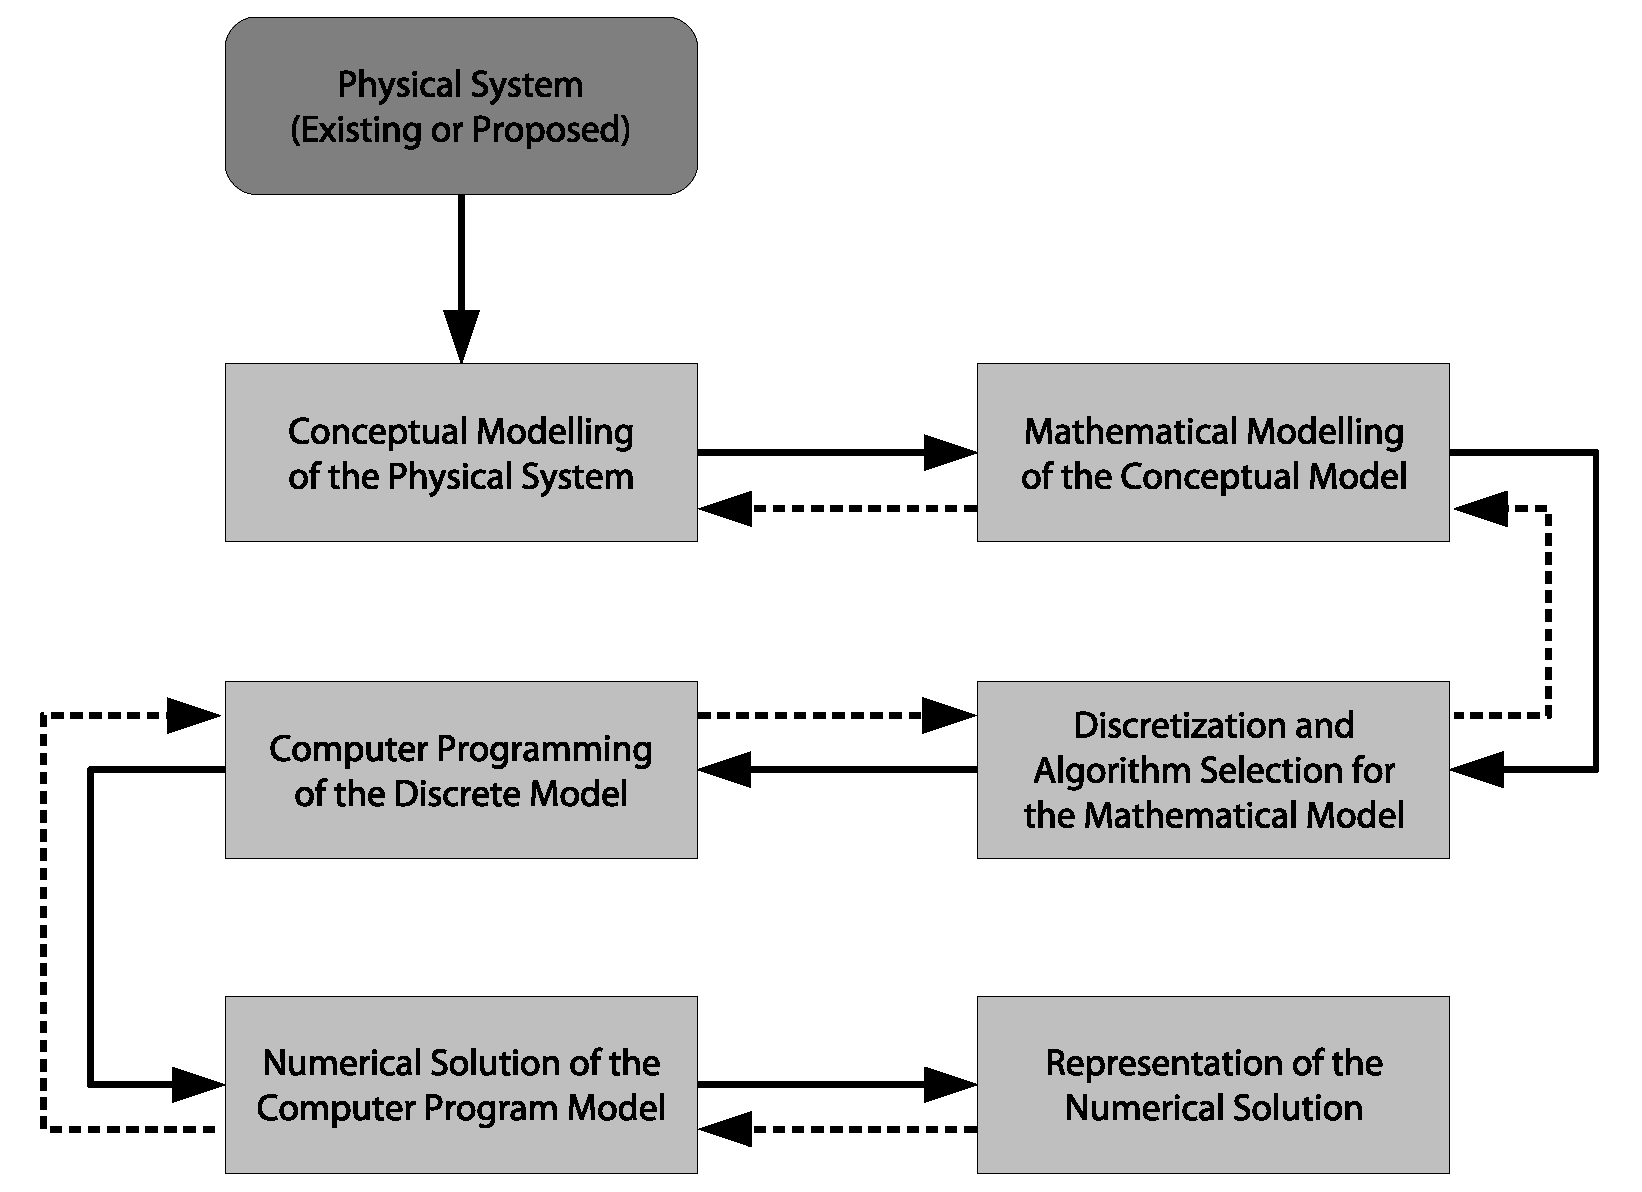
\includegraphics[width=0.90\textwidth]{./img/modelling_phases}
\caption[Proposed phases for computational modelling and simulation.]{Proposed
phases for computational modelling and simulation.
\citep[From][]{oberkampf2002-333}}
  \label{fig:modelling_phases}
\end{figure}

This framework is a synthesis of the reviewed literature, with three substantial
additions compared to a more conventional viewpoint. First, it makes a more
precise distinction between the system and the environment. Second, it places
more emphasis on the distinction between aleatory and epistemic uncertainty in
the analysis. Third, it includes a dominant element in the simulation of complex
physical processes; the numerical solution of non-linear Partial Differential
Equations (PDFs).

\paragraph{Conceptual modelling of of the physical system}
Conceptual issues are considered determining all possible factors.

\paragraph{Mathematical modelling of the conceptual model}
The primary activity of this phase is to develop detailed and precise
mathematical models. The complexity of the models depends on the physical
complexity of each phenomenon being considered, the number of physical phenomena
considered, and the level of coupling of difficult types of physics. Emphasis on
comprehensiveness in the mathematical model should not be interpreted as an
emphasis on complexity of the model. The predictive power of a model depends on
its ability to correctly identify the dominant controlling factors and their
influences, not upon its completeness or complexity. A model of limited, but
known, applicability is often more useful than a more complete model. Any
mathematical model, regardless of its physical level of detail, is by definition
a simplification of reality.

\paragraph{Discretization and algorithm selection for the mathematical
model}
Converting the mathematical models into a form that can be addressed through
computational analysis. Conversion of the continuum mathematics form of the
mathematical model into a discrete, or numerical, model. Specifying the
methodology that dictates which computer runs will be performed in a later phase
of the analysis to accommodate the non-deterministic aspects of the problem.

\paragraph{Computer programming of the discrete model---modular approach}
Algorithms and solution procedures defined in the previous phase are converted
into a computer code.

\paragraph{Numerical solution of the computer program model}
The individual numerical solutions are actually computed.

\paragraph{Representation of the numerical solution}
The representation and interpretation of both the individual and collective
computational solutions. Basically this phase concerns how to present results
for a group of specific audiences.

The erosion models used in the present research are reviewed in the next
section. However, an additional model, the Universal Soil Loss Equation (USLE),
is first discussed since this model embodies the basic concepts underpinning
many more recent models.

\subsection{Universal Soil Loss Equation (USLE)}
\label{sec:UniversalSoilLossEquationUSLE}

The first attempt to develop a soil loss equation for hillslopes was that of
\citet{zingg1940-59}, who related erosion to slope steepness and slope length.
Further developments led to the addition of a climatic factor based on the
maximum 30-minute rainfall total with a 2-year return period
\citep{musgrave1947-133}, a crop factor to take account of the
protection-effectiveness of different crops, a conservation factor and a soil
erodibility factor, consecutively. All these factors were then incorporated
together, modified and up-dated to the Universal Soil Loss Equation (USLE)
\citep{wischmeier1978-537}.

The USLE consists of six factors, which are simply multiplied together to
estimate soil loss although there is substantial interdependence between the
variables \citep{wischmeier1978-537}:
\begin{equation}
\label{eq:usle}
  A = R \times K \times LS \times C \times P
\end{equation}
where $A$ (tonnes$\cdot$ha$^{-1}$ yr$^{-1}$) is average annual soil loss, $R$
(MJ$\cdot$mm$\cdot$hr$^{-1}$ ha$^{-1}$ yr$^{-1}$) is rainfall erosivity, $K$
(t$\cdot$hr$\cdot$MJ$^{-1}$ mm$^{-1}$) is soil erodibility, $L$ (dimensionless
ratio) is the slope-length factor, $S$ (dimensionless ratio) is the
slope-steepness factor, $C$ (dimensionless ratio) is the cropping factor, and
$P$ (dimensionless ratio) is the conservation practice factor.

%
The rainfall erosivity factor ($R$) is related to the raindrop impact effect.
$R$ factor provides relative information on the amount and rate of runoff
associated with the rain. The soil erodibility factor ($K$) is used to represent
the differences of natural resistances of soils to erosion. The slope length
($L$) and steepness($S$) factors provide the topographic information that can
affect the rate of energy dissipation. The cropping factor ($C$) is the ratio of
soil loss from cropped field under specific conditions to the corresponding loss
from tilled, continuous fallow conditions. The conservation practice factor
($P$) is the ratio of soil loss with a specific conservation practice to the
corresponding loss with conventional slope tillage.
%

The USLE uses the empirical results of erosion studies conducted at many
locations over nearly a half-century of research, including rainfall erosivity,
soil erodibility, slope length, slope steepness, cropping and management
techniques, and supporting conservation practices of more than 10,000 plot-years
of data from about 50 locations in 24 states in the US
\citep{wischmeier1978-537}. The results were statistically analysed and the
relationships between the factors incorporated into equation \ref{eq:usle}.

Both the strength and weakness of the USLE lie in its estimation of erosion as
the product of a series of terms for rainfall, slope gradient, slope length,
soil, and cropping factors. However, it does not account for any non-linear
interactions between the factors \citep{wischmeier1978-537,meyer1984-99}.

\citet{nicks1998-377} suggests that USLE may be used to estimate soil loss on a
storm by storm basis where incremental rainfall is available. Rainfall erosivity
index ($EI$) for a rainfall event is calculated by
\begin{equation}
\label{eq:usleerosivityindex}
  EI=R_{0.5} \sum(210+89\,log_{10} I)
\end{equation}
where $I$ is the incremental rainfall intensity and $R_{0.5}$ is the maximum
storm 30 minutes rainfall.
Individual storm erosion amounts may then be calculated with the USLE using this
$EI$ value to replace the $R$ factor in equation \ref{eq:usle}, summed to give a
yearly soil loss, and then averaged to produce a mean annual erosion estimate.

In contrast, \citet{kinnell2005-851} points out important problems of predicting
event erosion using the USLE. One of the main problem described is that, in the
USLE, there is no direct consideration of runoff even though erosion depends on
sediment being discharged with flow, which varies with runoff and sediment
concentration. \citet{kinnell2005-851} concludes that the failure to consider
runoff as a primary factor in the USLE is the factor that causing the USLE to
produce the erroneous prediction of event erosion, which in turn leads to
systematic errors in predicting average annual soil loss.

Since the introduction of the USLE to estimate soil loss, it has become the
conservationists' primary tool for planning purposes
\citep{diaz1987-189,centeri2002-211}. The USLE provides an ease of use and
relatively reliable results, and requires only readily obtainable information in
order to estimate average annual soil loss. However,
\citet{wischmeier1976-misuse} warned about the problem of the misuse of the
USLE.

The database for the original USLE is restricted to the US east of the Rocky
Mountains \citep{wischmeier1978-537}. The base is further restricted to slope
where cultivation is permissible, normally 0 to 7\textdegree, and to soils with
a low content of montmorillonite; it is also deficient in information on the
erodibility of sandy soils \citep{wischmeier1978-537}. It is important to note
that, because the USLE was designed to estimate average annual soil loss from
any specific field over an extended period, soil loss estimates for a specific
year may substantially differ from the long-term average predicted by the
equation \citep{wischmeier1976-misuse}. Extrapolating the relationship beyond
the database for the original USLE, therefore, should be conducted with care.

The basic concepts of the USLE were subsequently used and developed by some
continuous simulation models. Some of these models are CREAMS (Chemicals,
Runoff, Erosion, and Agricultural Management Systems) \citep{knisel1980-creams},
EPIC (Erosion-Productivity Impact Calculator) \citep{williams1984-129}, SWRRB
(Simulator for Water Resources in Rural Basins) \citep{williams1985-970}, WEPP
(Water Erosion Prediction Project) \citep{nearing1989-1587, flanagan1995-usda}.

\subsection{Water Erosion Prediction Project (WEPP)}
\label{sec:WaterErosionPredictionProjectWEPP}

WEPP (Water Erosion Prediction Project) is a process-based model that describes
the processes, such as infiltration and runoff, soil detachment, transport,
deposition, plant growth, senescence, and residue decomposition, that lead to
erosion \citep{flanagan1995-usda}. The model takes four input files, climate,
soil characteristic, slope, and crop management.

WEPP was developed by the USDA-ARS (United States Department of
Agriculture-Agricultural Research Service) as a new-generation water erosion
prediction technology for the routine assessment of soil erosion for soil and
water conservation and environmental planning and assessment
\citep{flanagan2007-1603}. The development of WEPP was initialized with an
intention to replace the `long-used' USLE (See Section
\ref{sec:UniversalSoilLossEquationUSLE}) \citep{nearing1989-1587,
flanagan1995-usda}. WEPP no longer relies on factor values from the USLE,
instead uses separate erodibility parameters for interrill ($K_i$) and rill
erosion ($K_r$) \citep{flanagan1995-usda}. In WEPP, rills are assumed to have a
uniform rectangular cross-section with a uniform spacing of 1 metre. All rills
are assumed to be equally hydrologically efficient \citep{flanagan1995-usda}.

The steady state erosion component of WEPP is based on:
\begin{equation}
\label{eq:weppsedimentload}
  \frac{dG}{dx} = D_f+D_i
\end{equation}
where $G$ represents sediment load, $x$ is the distant downslope, $D_f$ is the
rill erosion rate, and $D_i$ is the interrill erosion rate. $D_f$ and $D_i$ are
calculated on a per rill area basis. Rill erosion, $D_f$, is positive for
detachment and negative for deposition, and calculated by:
\begin{equation}
\label{eq:wepprillerosionrate}
  D_f=D_c(1-\frac{G}{T_c})
\end{equation}
where $T_c$ is the transport capacity of flow in the rill, and $D_c$ is
detachment capacity of the rill flow and:
\begin{equation}
\label{eq:weppdetachmentcapacity}
  D_c=K_r(\tau_f-\tau_c)
\end{equation}
where $K_r$ is rill erodibility parameter, $\tau_f$ is flow shear stress acting
on soil particles, and $\tau_c$ is the critical shear stress or rill detachment
threshold parameter of the soil.
Interrill erosion is given by:
\begin{equation}
\label{eq:weppinterrillerosionrate}
  D_i=K_i I_e \sigma_{ir} SDR_{RR} F_{\textrm{\scriptsize nozzle}}
\frac{R_s}{\omega}
\end{equation}
where $K_i$ is the interrill erodibility, $I_e$ is the effective rainfall
intensity, $\sigma_{ir}$ is the interrill runoff rate, $SDR_{RR}$ is the
sediment delivery ratio, $F_{\textrm{\scriptsize nozzle}}$ is an adjustment
factor to account for sprinkler irrigation nozzle impact energy variation, $R_s$
is the rill spacing, and $\omega$ is the width. Interrill erosion is also
expressed with baseline interrill erodibility as \citep{nicks1998-377}:
\begin{equation}
\label{eq:weppinterrillerosionratealternative}
  D_i=K_{ib} I_e^2 C_C C_G \frac{R_s}{\omega}
\end{equation}
where $K_{ib}$ is baseline interrill erodibility, $C_C$ is the effect of canopy
cover on interrill erosion, and $C_G$ is the effect of ground cover on interrill
erosion. The hydrologic variables that drive the WEPP are the effective rainfall
intensity and duration, the peak runoff rate, and the effective runoff duration.

The USLE erosion database could not be used directly for the WEPP
parametrisation. Three field experiments on cropland, rangeland and forestland
were conducted to determine parameters for $K_r$ and $K_{ib}$ given in equations
\ref{eq:weppinterrillerosionrate} and
\ref{eq:weppinterrillerosionratealternative}. A total of 77 sets of plot data
were collected \citep{nicks1998-377}. Fixed rainfall intensity was applied to
the plots using a rainfall simulator. A comprehensive model description is
available in \citet{flanagan1995-usda}.

Rainfall is represented in the WEPP with the double exponential function. A
storm is described with four parameters, storm amount, average intensity, ratio
of peak intensity to average intensity, and time to peak intensity. A stochastic
weather generator, CLIGEN (CLImate GENerator; \citealp{nicks1995-2}) is used to
generate these storm precipitation inputs. More about CLIGEN is covered later in
Section \ref{sec:ClimateGeneratorCLIGEN}. WEPP then disaggregates these storm
inputs into a single peak storm intensity pattern (time-rainfall intensity
format) for use by the infiltration and runoff components of the model.
\citep{flanagan1995-usda}.

The WEPP model can be used for hillslope erosion processes (sheet and rill
erosion), as well as simulation of the hydrologic and erosion processes on small
watersheds. The hillslope mode predicts soil erosion from a single hillslope
profile of any length. It can be applied to areas up to about 260 hectares in
size. The watershed mode links hillslope elements of specified widths together
with channel and impoundment elements. WEPP is designed to run on a continuous
simulation but can also be operated for a single storm. A modified version of
the hillslope WEPP has been developed for research purposes
\citep{favis-mortlock1999-329,favis-mortlock1996-529}. This is designed to
account for the effects of atmospheric CO$_2$ concentration changes on plant
growth.

In this research, only hillslope mode of the WEPP (v2004.7) was used for
continuous or single-event simulation, depending on the purpose.

\subsubsection{CLIGEN}
\label{sec:ClimateGeneratorCLIGEN}
CLIGEN is a stochastic weather generator, which generates daily time series
estimates of precipitation, temperature, dew point, wind, and solar radiation
for a single geographical point, based on average monthly measurements for the
period of climatic record \citep{nicks1995-2}. The estimates for each parameter
are generated independently of the others \citep{nicks1995-2}.

In comparison to other climate generators, CLIGEN is better at preserving the
low-order statistics of rainfall, temperature, and solar radiation on a daily,
monthly, and annual basis \citep{nicks1995-2}. Unique to CLIGEN is the capacity
to simulate the three additional weather variables to characterize the storm
pattern, namely storm duration, time to peak, and peak intensity, which are
specifically developed for the WEPP simulation \citep{flanagan1995-usda}.

CLIGEN stochastically generates four precipitation-related variables for each
wet day, which are precipitation amount  (mm), $R$, storm duration (hour), $D$,
time to peak as a fraction of the storm duration, $t_p$, and the ratio of peak
intensity over average intensity, $i_p$. Average intensity is defined as $R/D$.
Although it is possible to calculate individual variables manually for each
rainfall event, it is a labour intensive task to calculate the variables for
multiple events.

CLIGEN requires observed precipitation statistics in order to generate these
four precipitation-related variables (Table
\ref{tab:PrecipitaionParametersRequiredByCLIGEN}).

\begin{table}[htbp]
  \centering
  \caption[Precipitation parameters required by CLIGEN]{Precipitation
parameters required by CLIGEN to generate WEPP precipitation inputs (from
personal communication with Bofu Yu, 2003)}
  \label{tab:PrecipitaionParametersRequiredByCLIGEN}
  \footnotesize
    \begin{tabular}{ll}
    \toprule
    \textbf{Parameter} & \textbf{Description} \\
    \midrule
    meanP & Average precipitation (inches) on wet days for each
month\\
    sdP & Standard deviation of daily precipitation (inches) for
each month\\
    skP & Coefficient of skewness of daily precipitation (inches)
for each month\\
    P(W/W) & Probability of a wet day following a wet day for each
month\\
    P(W/D) & Probability of a wet day following a dry day for each
month\\
    {MX.5P} & Average maximum 30-min peak intensity (in/hr) for each
month\\
    TimePk & Cumulative distribution of time to peak as a fraction
of the storm duration\\
    \bottomrule
    \end{tabular}
\end{table}

Precipitation data required to derive the CLIGEN input parameters in Table
\ref{tab:PrecipitaionParametersRequiredByCLIGEN} are time series of daily
precipitation data and sub-daily precipitation data with a time intervals no
greater than 30 minutes (personal communication with Bofu Yu, 2003). In
principle, there is no need to distinguish these two types of precipitation data
because sub-daily data can be accumulated to produce daily values. In practice,
however, these two types of data usually come from two different sources. The
coverage of the daily data, both in space and time, is much more extensive in
comparison to sub-daily data at short time intervals. In addition, the two types
of data are normally stored in different formats. It is therefore useful to
treat the two types of precipitation data separately.

CLIGEN (version 4.2) was previously released with WEPP version 2001.3. However,
this version of CLIGEN had a major coding error and was modified substantially
\citep{yu2000-301}. CLIGEN (version 4.2) computed a ratio $\omega = R_{0.5}/R$,
where both $R_{0.5}$ and $R$ were rainfall depth (originally in inches).
$R_{0.5}$ had been converted from inches into millimetres (mm), while $R$ was
not \citep{yu2000-301}. The CLIGEN code was thus changed to correct this error.
This however led to extensively increased storm durations.

To accommodate the correction of unit conversion error, it was necessary to
incorporate two important modifications in the CLIGEN codes. First, a new
algorithm to determine the monthly means of the maximum 30-min rainfall depth
was implemented. Secondly, the parameter values for storm duration and the
coefficient of variation for the ratio of the maximum 30-min rainfall depth to
daily rainfall required in CLIGEN were estimated using the break-point rainfall
data \citep{yu2000-301}.

This error in the CLIGEN code has certainly affected the results from the
earlier studies, which employed the previous versions of WEPP and CLIGEN to
estimate soil loss
\citep{truman1993-405,zhang1995-1069,zhang1995-1079,zhang1996-855,
baffaut1996-447,laflen1997-96,baffaut1998-756,favis-mortlock1999-329}.

The version of CLIGEN at the time of writing is version
5.22564\footnote{http://horizon.nserl.purdue.edu/Cligen/, April 2006}. This is
the version used in this research.


\subsection{European Soil Erosion Model (EUROSEM)}
\label{sec:EuropeanSoilErosionModelEUROSEM}

EUROSEM is a dynamic distributed event-based model for simulating erosion,
transport and deposition of sediment over the land surface by interrill and rill
processes \citep{morgan1998-389}. The model has explicit simulation of interrill
and rill flow; plant cover effects on interception and rainfall energy; rock
fragment effects on infiltration, flow velocity and splash erosion; and changes
in the shape and size of rill channels as a result of erosion and deposition
\citep{morgan1998-389}. It can be applied to a small field and up to a small
catchment.

EUROSEM requires a one-minute resolution breakpoint rainfall data for the storm.
The model then computes, using the breakpoint rainfall data, the interception of
the rain by the plant cover, the generation of runoff as infiltration excess,
soil detachment by raindrop impact, soil detachment by runoff, transport
capacity of the runoff and deposition of sediment. The model has a modular
structure that aims to make further improvements of the model easier. The model
considers the followings:
\begin{itemize}
\item the interception of rainfall by the plant cover
\item the volume and kinetic energy of the rainfall reaching the ground surface
as direct throughfall and leaf drainage
\item the volume of stemflow
\item the volume of surface depression storage
\item the detachment of soil particles by raindrop impact and by runoff
\item sediment deposition
\item the transport capacity of the runoff
\item frozen soils and stoniness
\end{itemize}

The flow chart for EUROSEM is shown in Figure \ref{fig:eurosem_flow_chart}.

\begin{figure}[htbp]
  \centering
    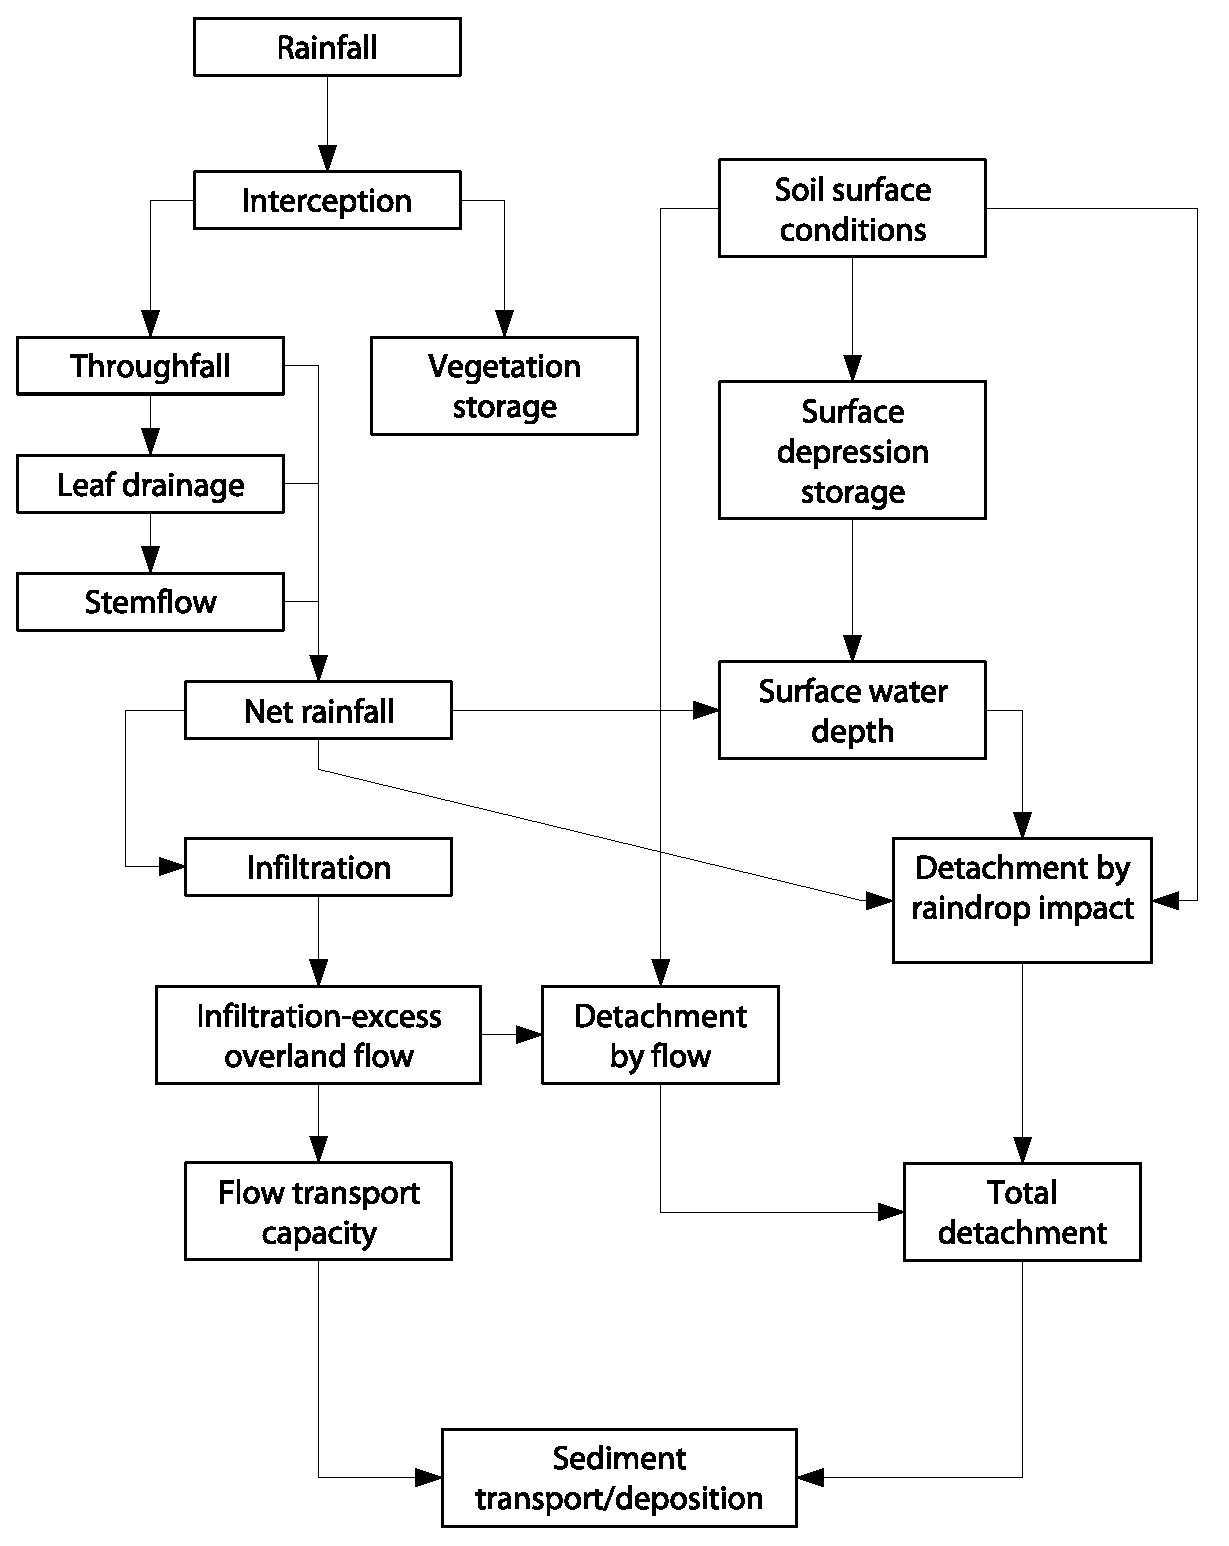
\includegraphics[width=0.80\textwidth]{./img/eurosem_flow_chart}
  \caption[Flow chart of EUROSEM]{Flow chart of EUROSEM (from
\citealp{morgan1998-389})}
  \label{fig:eurosem_flow_chart}
\end{figure}

Runoff generator and the water and sediment routing routines of EUROSEM are from
another model called KINEROS \citep{woolhiser1990-kineros}. The volume of
sediment passing a given point on the land surface at a given time is calculated
by a mass balance equation:
\begin{equation}
\label{eq:eurosemmassbalance}
  \frac{\partial(AC)}{\partial t}+\frac{\partial(QC)}{\partial x}-e(x,t)=
q_s(x,t)
\end{equation}
where $C$ is sediment concentration (m$^3$/m$^3$), $A$ is the cross sectional
area of the flow (m$^2$), $Q$ is the discharge (m$^3$/s), $q_s$ is external
input or extraction of sediment per unit length of flow (m$^3$ s$^{-1}$
m$^{-1}$), $e$ is net detachment rate or rate of erosion of the bed per unit
length of flow (m$^3$ s$^{-1}$ m$^{-1}$), $x$ is horizontal distance (m), and
$t$ is time (s).
The net detachment rate, $e$, is given as:
\begin{equation}
\label{eq:eurosemnetdetachmentrate}
  e = DR + DF
\end{equation}
where $DR$ is the rate of soil particle detachment by raindrop impact (m$^3$
s$^{-1}$ m$^{-1}$), and $DF$ is the balance between the rate of soil particle
detachment by the flow and the particle deposition rate (m$^3$ s$^{-1}$
m$^{-1}$).

The EUROSEM simulates erosion and deposition by calculating three main
processes, soil particle detachment by raindrop impact, soil particle detachment
by runoff, and transport capacity of the flow.

\paragraph{Soil particle detachment by raindrop impact}
\label{sec:SoilParticleDetachmentByRaindropImpact}
Soil detachment by raindrop impact ($DR$) for time step ($t_s$) is expressed as
a function of the kinetic energy of the rainfall at the ground surface, the
detachability of the soil and the surface water depth:
\begin{equation}
\label{eq:EUROSEMsoildetachmentbyraindropimpact}
  DR = \frac{k}{\rho_s} {KE} e^{-zh}
\end{equation}
where $k$ is an index of the detachability of the soil (m$^3$/J), $\rho_s$ is
the sediment particle density (=2.65 Mg/m$^3$), $KE$ is the total kinetic energy
of the net rainfall at the ground surface (J/m$^2$), $z$ is an exponent taken as
equal to 2.0 which varies between 0.9 and 3.1 \citep{torri1987-149}, and $h$ is
the mean depth of the surface water layer (m).
The kinetic energy of the rainfall is the combined energy from direct
throughfall and leaf drainage. The energy of the direct throughfall is computed
using raindrop size distribution found by \citet{marshall1948-165}. The energy
of the leaf drainage is based on a study by \citet{brandt1990-687}.

\paragraph{Soil particle detachment by runoff}
\label{sec:SoilParticleDetachmentByRunoff}
Soil particle detachment by runoff is based on a theory proposed by
\citet{smith1995-517}, and is given as:
\begin{equation}
\label{eq:eurosemsoilparticledetachmentbyrunoff}
  DF = \beta w v_s (TC-C)
\end{equation}
where $DF$ is the rate of detachment of soil particles by the flow, $\beta$ is a
flow detachment efficiency coefficient ($\beta=1$ when deposition is taking
place and $\beta < 1$ for cohesive soils when $DF$ is positive), $w$ is the
width of the flow (m), $v_s$ is the setting velocity of the particles in the
flow (m/s), $TC$ is the sediment concentration in the flow at transport
capacity, and $C$ is the actual sediment concentration in the flow.

\paragraph{Transport capacity of flow}
\label{sec:TransportCapacityOfTheFlow}
EUROSEM uses two separate transport capacity relationships for rill and
interrill flows. Rill and interrill transport capacities are based on
\citet{govers1990-45} and \citet{everaert1991-513}, respectively. The equation
for rill transport capacity ($TC_{r}$) is expressed as:
\begin{equation}
\label{eq:EUROSEMRillTransportCapacity}
  TC_{r} = c(\omega - \omega_c)^{\eta}
\end{equation}
where $\omega$ is unit stream power (cm/s) which is defined as $\omega = 10
\upsilon s$ ($\upsilon$ = mean flow velocity (m/s) and $s$ = slope (\%)),
$\omega_c$ is a critical value of unit stream power (0.4 cm/s), and $c$ and
$\eta$ are experimentally derived coefficients related to the median particle
size of the soil.
Interrill transport capacity ($TC_{ir}$) is modelled as:
\begin{equation}
\label{eq:EUROSEMInterrillTransportCapacity}
  TC_{ir} = \frac{b}{\rho_s q}\left[(\Omega -
\Omega_c)^{\frac{0.7}{n}}-1\right]^{\kappa}
\end{equation}
where $b$ is a function of particle size, $\rho_s$ is the sediment density
(Kg/m$^3$), $\Omega$ is Bagnold's modified stream power, $\Omega_c$ is a
critical value of Bagnold's modified stream power, $n$ is Manning's $n$, and
$\kappa$ = 5. Sediment delivery to the rills is simulated depending on the
transport capacity of the interrill flow.

Since EUROSEM uses a dynamic rather than steady-state approach used by WEPP, it
gives a better understanding of the spatial and temporal distribution of runoff
and erosion. However, the result of the model simulation may become considerably
uncertain due to its process-based nature that requires detailed model
parametrization \citep{quinton1998-65}. Particularly, EUROSEM requires high
resolution rainfall data (ideally, 1-min breakpoint data), soil hydrological
information, detailed surface geometry, and soil mechanical and vegetation
characteristics. Because of the detailed requirements of the model, application
of the model is greatly restricted to where such data are available.

\citet{parsons2000-181} found that because EUROSEM ignores small-scale
heterogeneities in the infiltration characteristics of soil, the model generates
delayed initiation times for runoff, so that predicted hydrographs showed the
commencement of runoff later than observed. Such variabilities in the
infiltration characteristics may be responsible for the comparatively rapid
initiation of runoff on the plot. They also found that the subsequent soil
detachment by runoff in interrill areas is overestimated by the model even
though, according to the model document, detachment by flow should be negligible
in interrill areas.

After personal communication (16 Jun 2004) with Anthony J. Parsons , it is noted
that EUROSEM may have a unit conversion error. The model document states that
the flow depth ($h$) in equation \ref{eq:eurosemsoilparticledetachmentbyrunoff}
is in metres. However, a study by \citet{torri1987-149} on which this equation
is based indicates that the height is in millimetres (see Figure 2 in
\citet{torri1987-149}). Anthony J. Parsons suggests that the height is in
centimetres rather than either metres or millimetres. If confirmed, this error
would have major effects on EUROSEM's ability to estimate runoff and erosion.

%First does the storm pattern affect the  runoff coefficient (same amount of
%rain but different amount of runoff) so  do differences in erosion result
%simply from more or less runoff?
%Secondly,  does the intensity pattern affect detachment so you get more or
%less erosion  because of the detachment effect.  We have something to say
%about that (sort of) in a paper in ESPL that should appear at some point
%(when I submit it!).
%So I think Mintae needs to look carefully at what is happening in the 2
%models in terms or runoff coefficients and detachment rates.

The version of EUROSEM used in this research is 3.9 (14/12/1998), which is the
current version of the model. It seems that the model development has been
ceased for some time.
%It may have been the case that the model developer have abandoned the model.

\subsection{RillGrow}
\label{sec:ModelDescriptionRillGrow}

While the later two erosion models (i.e. WEPP and EUROSEM) reviewed previously
are capable of realistically simulating rates of soil erosion, they (in common
with all other present-day erosion models) have a number of conceptual
shortcomings. For example, rills are considered to be equally spaced, with
regular cross-sections, and to be of similar hydrological efficiency. In
reality, rills are not necessarily spaced regularly and often have irregular
cross-sections. Adjacent rills may also vary greatly in their ability to
transport runoff and sediment \citep{favis-mortlock1996-248}. Additionally,
while such models separately describe the different processes responsible for
erosion in rill and interrill areas, they largely fail to acknowledge the
physical link that exists between the processes operating in the two zones
\citep{favis-mortlock2000-2173}.

The development of the RillGrow model
\citep{favis-mortlock1996-248,favis-mortlock1998-353,favis-mortlock2000-2173,
favis-mortlock2003-127,favis-mortlock2004-349} started with a consideration of
these shortcomings, and a question `\emph{Is the initiation and development of
hillslope rill systems driven by relatively simple rules acting on a much
smaller scale?}'. To test this hypothesis, a self-organising dynamic systems
approach was used to simulate the initiation and development of a rill network
on the bare soil of a small (e.g.\ plot-sized) hillslope area.

RillGrow is a single-event model, which generates realistic rill networks by
simulating, on a grid of microtopographic elevations, the combined erosive
action of overland flow moving between the cells of the grid. Surface water
arrives, a single raindrop at a time, on random cells of the grid. Runoff moves
over the grid following the steepest microtopographic gradient; as it moves, it
erodes the soil surface by lowering the elevation of the soil's surface. Each
change in elevation affects the routing of subsequent runoff: the result is a
feedback loop in which flow patterns over the grid at any time depend on earlier
flow patterns (and hence erosion), these flow patterns then condition subsequent
flow patterns, and so on (Figure \ref{fig:rillgrow_feedback_concept}).

\begin{figure}[htbp]
  \centering
    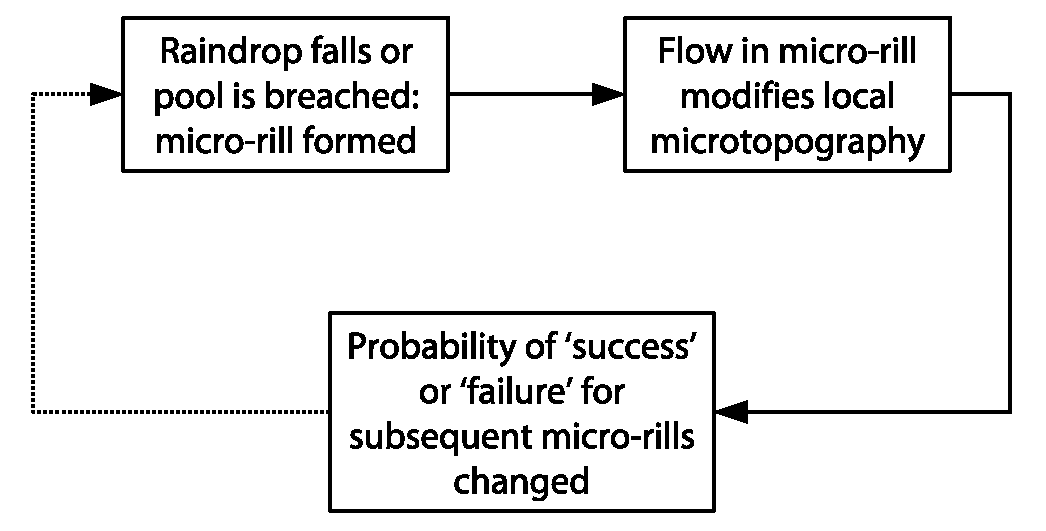
\includegraphics[width=0.80\textwidth]
{./img/rillgrow_feedback_concept}
  \caption[The conceptual feedback loop of RillGrow]{The conceptual
feedback loop of RillGrow \citep[From][]{favis-mortlock1998-353}}
  \label{fig:rillgrow_feedback_concept}
\end{figure}

The first version of the RillGrow model was able to realistically simulate rill
initiation and development, reproducing several features of observed rill
systems \citep{favis-mortlock1996-248,favis-mortlock1998-353}:
\begin{enumerate*}
  \item a narrowing of rill spacing with increased slope angle
  \item an increased contribution of rill erosion with downslope distance
  \item a non-linear increase of total erosion with slope steepness
  \item an increase in rill depth below confluences and micro-rill piracy
\end{enumerate*}

However, RillGrow 1 has some important limitations. It ignores important process
descriptions (e.g.\ infiltration, deposition), and the hydraulics of rill
initiation are oversimplified. It also does not operate in a true time domain,
since at any moment during the simulation, only a single `packet' of overland
flow is moving over the topographic grid. Infiltration is ignored, thus all
water on the grid is assumed to be rainfall excess, and transport capacity is
assumed to be infinite because no deposition can occur
\citep{favis-mortlock2000-2173}.
All these limitations meant that it was not possible to validate the model in a
deterministic way, e.g. by comparing simulated and laboratory-produced rill
networks.

A second version of the model (`RillGrow 2') was developed to overcome some of
these limitations, and allow more rigorous validation
\citep{favis-mortlock2000-2173}. In RillGrow 2, overland flow in effect moves
concurrently between cells of the
microtopographic grid. Such concurrency is not easy to achieve on a
serial-processing computer, since only one instruction can be carried out at a
time. Concurrent processing is simulated in RillGrow 2 in the following way:
during a given timestep, outflow from each `eligible' wet cell is routed in a
random sequence which differs for each timestep. This variation in sequence is
necessary to prevent any artefacts of flow pattern which might result from a
fixed routing sequence. Over a sufficient number of timesteps, the model in
effect operates in `parallel', i.e. concurrently, in a true time domain.

\begin{table}[htb]
  \centering
  \small
  \caption[The main routing algorithm used in RillGrow 2]{The main routing
algorithm used in RillGrow 2 \citep[From][]{favis-mortlock2000-2173}. Note that,
while
this set of rules does not change during the model simulation, the result of
applying the rules to a given cell depends on the past history of elevation
change both for that cell, and for adjacent ones.}
  \label{tab:TheMainRoutingAlgorithmUsedInRillGrow2}
    \begin{tabular}{p{0.9\textwidth}}
    \toprule
For each iteration:\\
\\
Drop raindrops on random cells on the spatial grid. Each drop makes (or adds to,
if the cell is already `wet') a store of surface water for that cell.\\
\\
Go through all `wet' cells in a random sequence (which is different each
iteration). For each `wet' cell, check whether sufficient time has elapsed for
flow to have traversed the cell. If it has, then do the following:\\
\begin{itemize}
  \item Find the adjacent cell which has the steepest downhill (i.e.\
outflow) energy gradient. Note that this adjacent cell may or may not be already
`wet'.
  \item Attempt to level the energy gradient between these cells by
outflow of an appropriate volume, adding to (or creating) the store of surface
water on the adjacent cell.
  \item Erode this cell (i.e.\ lower its soil-surface elevation) by an
amount which depends on the outflow volume and velocity.
  \item If there are other adjacent cells with downhill energy gradients,
process these as above.
\end{itemize}\\
%\addlinespace[-2mm]
    \bottomrule
    \end{tabular}
\end{table}

RillGrow 2 also uses a refined set of basic rules for the routing algorithm
(Table \ref{tab:TheMainRoutingAlgorithmUsedInRillGrow2}). A probabilistic
expression by \citet{nearing1991-81}, based on the random occurrence of
turbulent bursts, is used to represent flow detachment. Sediment load is
compared with transport capacity, which is calculated using stream power in an
s-curve expression developed by \citet{nearing1997-865}. Deposition is estimated
using the approach of  \citet{lei1998-3157}: this assumes deposition to be a
linear function of the difference between sediment load and transport capacity.

Infiltration is now simulated by RillGrow 2, however the approach used is still
very simple (Favis-Mortlock, personal communication 2006). Splash redistribution
is also represented, using the diffusion-based approach of
\citet{planchon2000-131}, modified to include attenuation due to surface water
depth (Favis-Mortlock, personal communication 2006). Additionally, a simple
linkage is made between overall volumes of sediment detached or deposited by
splash in any timestep, and volumes of sediment currently being transported by
overland flow (Favis-Mortlock, personal communication 2006). The distribution of
raindrop volumes is assumed to be normally distributed (Favis-Mortlock, personal
communication 2006).

In comparison to models such as WEPP and EUROSEM, RillGrow makes no explicit
separation between rill and interrill areas. Soil erosion amount is calculated
as the result of summation of soil losses from all areas.
%Explicit separation of rill and interrill areas turns out to be unnecessary,
%however.
Flow velocities are so low on interrill areas that little detachment occurs as a
result. On such areas, splash redistribution dominates.

\citet{favis-mortlock2000-2173} observes that RillGrow 2 replicates the
responses of RillGrow 1 including realistic rill spacing with respect to slope
gradient. In addition, the simulated spatial patterns of erosion compare well
with
laboratory-based observations, as do total erosion, variation in rill depth, and
time-series of runoff and soil loss. Braided or dendritic flow patterns can be
made to emerge by varying rainfall intensity. At low rainfall intensities,
however, the definition and stability of rill patterns is less well defined.

As originally constructed, RillGrow 2 assumed each storm to have a constant
rainfall intensity. For the research described in this thesis, RillGrow 2 has
been modified to use breakpoint rainfall data. This allows the model to simulate
rill initiation and development and total soil loss, as affected by rainfall
intensity changes (Favis-Mortlock, personal communication 2006).


%\nolinenumbers*
